\section{589 --- N-ary Tree Preorder Traversal}
Given an $n$-ary tree, return the \textit{preorder} traversal of its nodes' values.

For example, given a 3-ary tree:

\begin{figure}[H]
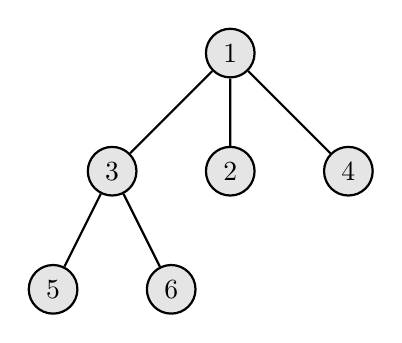
\begin{tikzpicture}
[every node/.style={draw, circle,minimum size=6mm, fill=gray!20!}, node distance=8mm,thick]
\node{1}
child{node{3} child{node{5}} child{node{6}}}
child{node{2}}
child{node{4}};
\end{tikzpicture}
\end{figure}

Return its preorder traversal as: $[1,3,5,6,2,4]$.


\paragraph{Note:}

\begin{itemize}
\item Recursive solution is trivial, could you do it iteratively?
\end{itemize}

\subsection{Stack}
\begin{itemize}
\item Iteration method is similar to binary tree, we insert the children nodes into the stack reversely.
\end{itemize}

\setcounter{lstlisting}{0}
\begin{lstlisting}[style=customc, caption={Stack}]
vector<int> preorder( Node* root )
{
    stack<Node*> stk;
    stk.push( root );

    vector<int> ans;

    while( !stk.empty() )
    {
        auto t = stk.top();
        stk.pop();

        if( !t )
        {
            break;
        }

        ans.push_back( t->val );

        if( t->children.empty() )
        {
            continue;
        }

        for( size_t i = 0; i < t->children.size(); ++i )
        {
            //put the childre per the reverse order
            //into the stack
            auto j = t->children.size() - i - 1;
            stk.push( t->children[j] );
        }

    }
    return ans;
}
\end{lstlisting}